% =====================================================================
%  InsightVLM — Thesis (Overleaf project)
%  Team Hocrux · Phitron AI/ML Thesis Track
%
%  Upload this whole folder to Overleaf (New Project -> Upload Project).
%  Compile with pdfLaTeX. Bibliography: BibTeX (references.bib).
% =====================================================================
\documentclass[12pt,a4paper]{report}

\usepackage[margin=2.5cm]{geometry}
\usepackage{times}
\usepackage{graphicx}
\usepackage{booktabs}
\usepackage{amsmath,amssymb}
\usepackage{url}
\usepackage[hidelinks]{hyperref}
\usepackage{caption}
\usepackage{multirow}
\usepackage{longtable}
\usepackage{enumitem}
\usepackage{xcolor}
\graphicspath{{figures/}}
\usepackage{tikz}
\usetikzlibrary{shapes.geometric,arrows.meta,positioning}
\usepackage[numbers,sort&compress]{natbib}

\sloppy
\emergencystretch=2em
\captionsetup{font=small,labelfont=bf}
\setlength{\parskip}{0.3em}

% Marker for anything that must be verified against a source before submission.
\newcommand{\verify}[1]{\textcolor{red}{\textbf{[VERIFY: #1]}}}

\title{\textbf{InsightVLM: Automated Statistical Reasoning\\from Data Visualizations}}
\author{Team Hocrux\\[0.4em]
A K M Asifuzzman \quad Robiul \quad Fahim Ali \quad Iftehad \quad Md Arfat Yunus\\[0.6em]
\textit{Phitron AI/ML Thesis Track}}
\date{\today}

\begin{document}
\maketitle

\begin{abstract}
\noindent
Charts carry most quantitative findings to their readers, yet chart-understanding
datasets supervise models to answer questions, describe figures or reconstruct code,
never to state what the data shows and be checked against it. This thesis introduces
\textbf{InsightVLM-20K}: 20{,}000 charts in 26 chart types, each labelled with one of 20
statistical findings (such as bimodality, heteroscedasticity, a level shift, or a
non-significant group difference) that a named statistical test has confirmed on exactly
the plotted data. 6{,}083 charts come from 654 real public tables in source-disjoint
splits, so generalisation to real data is measured directly.

A fine-tuned CNN ensemble names the finding of a real test chart with \textbf{0.867}
accuracy (95\% CI 0.846--0.886) and of a synthetic chart with 0.999, against 0.468 for the
best zero-shot vision--language model and 0.288 for a rule that uses no pixels. Accuracy
falls to 0.716 when the same real data is drawn by a plotting library never seen in
training; training on charts drawn by several libraries is the most effective remedy we
found. A QLoRA-tuned generative model names findings 80\% of the time but cites correct
numbers only 13.8\% of the time. A Grad-CAM pointing game shows the classifier's attention
falls on the verified evidence beyond chance for three of four finding families.

We also report two errors found and corrected along the way: label-dependent marks in
the renderer that had inflated time-series accuracy to 0.96 from a true 0.31--0.41, and an
ensemble selected on the test set. The dataset, the evaluation protocol, the trained
models and an interactive tester are released.
\end{abstract}

\tableofcontents

% ---------------------------------------------------------------------
%  Chapters are organised by the week they were produced.
%  main.tex and references.bib stay in the ROOT directory.
% ---------------------------------------------------------------------
\chapter{Introduction}
\label{ch:intro}

\section{Background}

Quantitative findings travel as pictures. A reader meets a distribution, a
correlation or a trend as a chart long before meeting the numbers behind it. The
properties that most often invalidate a naive reading --- bimodality that makes a
mean meaningless, heteroscedasticity that invalidates a standard error, a group
difference that is statistically significant yet practically negligible --- are
present in the figure but absent from its caption.

Recent Vision--Language Models (VLMs) are able to understand charts, answer
questions, generate descriptions, and reconstruct underlying data. However, most
existing approaches are designed for a predefined task and a user-specified
query, rather than for automatically discovering the important statistical
patterns in a visualization.

\section{Problem Statement}
\label{sec:problem}

Existing chart VLMs answer questions a human already thought to ask, describe
what a figure looks like, or reconstruct the code that drew it. None of these
objectives requires the model to decide \emph{what is worth reporting}.
Consequently users must still manually study a chart to determine its trends,
relationships, distributions and anomalies.

Three specific deficiencies follow, and they organise the rest of this thesis.

\paragraph{(P1) No corpus carries a verified \emph{statistical} finding as
ground truth.} Supervision in prior work is a question and an answer, a caption,
or plotting code. Recent work does verify factual claims about charts
\citep{chocolate,techrxiv}, but it does so \emph{post hoc}, on captions a model
has already produced, and at the level of values, labels and simple trends.
No corpus pairs each chart with a statistically confirmed finding that a model
could be \emph{trained} toward. Without such a label there is nothing to optimise
for statistical correctness, and a model may reconstruct a histogram's data table
perfectly while never observing that the distribution is bimodal.

\paragraph{(P2) Analysis is not question answering.} Autonomous analysis requires
choosing what to report. A model answering a supplied question never makes that
choice, so question-driven benchmarks cannot measure the capability we care
about.

\paragraph{(P3) Claims are ungrounded.} No chart corpus ties a stated finding to
the specific pixels that support it. The question ``was the model right for the
right reason?'' therefore cannot be asked, let alone answered. \citet{shortcut}
show why this matters: without such a check, a model may reach high accuracy
through features that carry no statistical evidence at all.

\paragraph{Who this affects.} Analysts and domain scientists who read charts under
time pressure and need the non-obvious property flagged; and anyone consuming
automated reporting built on current chart VLMs, where a fluent but statistically
wrong summary is indistinguishable from a correct one.

\section{Scope}

\paragraph{In scope.} Twenty statistical finding classes across four analysis
families (distribution shape, bivariate relationship, temporal behaviour, group
comparison); single-label classification and generation from a static chart
image; a balanced, statistically verified benchmark with underlying data tables,
supporting statistics and pixel-level evidence; charts rendered with
\texttt{matplotlib}/\texttt{seaborn} at fixed resolution.

\paragraph{Out of scope.} Compound findings (charts exhibiting two findings at
once were excluded rather than multi-labelled); causal claims; cross-renderer
generalisation to Excel, Plotly, D3 or hand-drawn figures; interactive, 3-D,
geographic and multi-panel dashboards; chart-type classification as an end in
itself.

\section{Motivation}

Two observations motivate the work.

First, \textbf{statistical correctness is not currently measurable} in this
field. A chart VLM can produce a fluent paragraph containing fabricated numbers
and score well on every existing benchmark, because those benchmarks grade
answers rather than claims. Our own experiments make this concrete: a fine-tuned
VLM names the correct finding in $80\%$ of cases while only $13.8\%$ of the
numbers it cites appear in the ground truth (Chapter~\ref{ch:method}).

Second, \textbf{numeracy failures have been documented only in text.}
Several authors show that language models struggle with statistical operations
\citep{stateval,numericbench,numeracynli,bittokens}, but every such evaluation
supplies the numbers directly. Whether the weakness persists when a number must
first be read off a rendered chart is untested.

Third, \textbf{synthetic chart corpora are now standard, and their
generalisation is rarely measured.} Large-scale synthetic generation has become
the dominant way to scale chart datasets, but without a held-out real subset it
is impossible to say how much reported performance is a generator artefact.

\section{Research Questions}
\label{sec:rqs}

\begin{description}[leftmargin=1.6cm,style=nextline,font=\bfseries]
  \item[RQ1.] Can a vision--language model be trained to automatically identify
  statistical patterns, including trends, correlations, distribution
  characteristics and anomalies, directly from a chart image without a supplied
  question?

  \item[RQ2.] How does the statistical correctness of VLM-generated insights
  compare with a deterministic rule-based statistical pipeline applied to the
  same underlying data?

  \item[RQ3.] To what extent do insights generated by InsightVLM remain
  evidence-grounded, meaning that each insight can be traced to a specific,
  verifiable statistical claim and its supporting chart evidence?

  \item[RQ4.] How well does a model trained primarily on synthetic chart data
  generalise to real-world charts, as measured on a held-out real-only
  evaluation set?

  \item[RQ5.] What evaluation protocol correctly measures statistical-pattern
  detection performance on chart images, given that chart type alone is
  structurally predictive of the finding class, and how robust is the underlying
  dataset to non-statistical shortcuts?
\end{description}

\section{Objectives}
\label{sec:objectives}

\begin{description}[leftmargin=1.2cm,style=nextline,font=\bfseries]
  \item[O1.] Build the multimodal chart dataset and statistical ground truth.
  \item[O2.] Train and evaluate InsightVLM for autonomous statistical-pattern
  detection.
  \item[O3.] Build the deterministic statistical baseline and compare
  correctness.
  \item[O4.] Develop the evidence-grounding evaluation.
  \item[O5.] Evaluate generalisation on real-world charts.
  \item[O6.] Define a corrected evaluation protocol (chart-type-prior floor,
  data-oracle ceiling) and audit the dataset for non-statistical shortcuts
  (caption text, chart-type bias, real/synthetic provenance leakage).
\end{description}

\begin{table}[t]\centering\small
\caption{Traceability. Every objective serves a research question and addresses a
deficiency from Section~\ref{sec:problem}; no objective exists without both.}
\label{tab:traceability}
\begin{tabular}{llll}
\toprule
\textbf{Objective} & \textbf{Serves} & \textbf{Addresses} & \textbf{Measured by} \\
\midrule
O1 & RQ1 & P1 & Label re-verification rate; generator$\rightarrow$class fidelity \\
O2 & RQ1 & P2 & Class accuracy; macro-F1 \\
O3 & RQ2 & P1 & Numeric fidelity vs.\ deterministic oracle \\
O4 & RQ3 & P3 & Evidence Pointing Accuracy vs.\ random control \\
O5 & RQ4 & P1 & Real-only probe vs.\ synthetic accuracy \\
O6 & RQ5 & P1, P2 & Chart-type prior; oracle ceiling; 11-test shortcut audit \\
\bottomrule
\end{tabular}
\end{table}

\section{Contribution Statement}
\label{sec:contribution}

\begin{enumerate}[leftmargin=1.4em]
  \item A purpose-built multimodal chart dataset pairing chart images with
  underlying tabular data and \emph{statistically verified} findings, providing a
  controlled foundation for evaluating autonomous statistical pattern discovery.

  \item \textbf{InsightVLM}, a vision--language approach designed to
  automatically identify and report statistical patterns and insights from chart
  images without requiring a predefined user question.

  \item A statistical-correctness evaluation framework that compares
  model-generated insights against a deterministic rule-based statistical
  pipeline operating on the same underlying data.

  \item An evidence-grounding evaluation protocol for determining whether
  generated insights can be traced to specific, verifiable statistical claims and
  supporting chart evidence.

  \item A generalisation evaluation measuring the performance of a model trained
  primarily on synthetic charts when evaluated on a held-out set of real-world
  charts.

  \item A corrected evaluation protocol establishing a chart-type-prior floor and
  a data-oracle ceiling for scoring statistical pattern detection, together with a
  shortcut and bias audit verifying that the dataset cannot be solved via
  non-statistical cues.
\end{enumerate}

\section{Thesis Structure}

Chapter~\ref{ch:lit} reviews the chart-understanding literature in seven groups
and identifies the gap this work targets. Chapter~\ref{ch:method} describes the
methodology: dataset construction and its verification gate, the models, the
evaluation protocol, and the risks that could invalidate the work.
Chapter~\ref{ch:results} reports the results, beginning with a correction to earlier
drafts (a rendering leak and a test-set selection), and answers each research question.
Chapter~\ref{ch:discussion} discusses what the results mean, the lessons of the leak,
threats to validity and limitations. Chapter~\ref{ch:conclusion} concludes and sets out
future work. Appendix~\ref{app:tester} describes the interactive tester and
Appendix~\ref{app:repro} lists the artefacts and how to regenerate every result.
      % Week 1: problem, RQs, objectives, contribution
\chapter{Literature Review}
\label{ch:lit}

This chapter reviews 23 papers grouped by \emph{what their supervision signal
actually is}, rather than by model architecture. That axis is chosen deliberately:
the central claim of this thesis concerns what a dataset teaches a model to do,
not how the model is built.

\section{Review Method}

Papers were selected to cover (i) the benchmarks that define chart understanding,
(ii) the largest and most recent chart corpora, (iii) the numeracy literature that
establishes where language models fail at statistics, (iv) the two works that
verify factual claims about charts, and (v) the methodological works that justify
our auditing practice. Each paper was read against a nine-question extraction
protocol covering problem, data, inputs, method, baselines, evaluation, results,
limitations and reproducibility. Seven groups emerged.

\section{Group 1: Chart Understanding and Recognition}

Several authors approach chart understanding as a structure-recovery problem.
\citet{pix2struct} pretrain on screenshot parsing with variable-resolution
inputs; \citet{matcha} add mathematical reasoning and chart derendering to that
pretraining, reaching $90.2$ relaxed accuracy on ChartQA; \citet{unichart}
introduce a chart-grounded pretraining corpus and reach $88.56$. \citet{charxiv}
then show that these gains are fragile on realistic charts drawn from scientific
papers.

The shared limitation is that all four target \emph{recognition}. They recover
what a chart shows --- values, axes, structure --- and answer questions about it.
None proposes a statistical characterisation of the data on its own initiative.

\section{Group 2: Chart Question Answering}

Several authors established chart QA as a task by generating questions over
figures: \citet{figureqa} and \citet{dvqa} from templates over synthetic
charts, \citet{plotqa} over scientific plots with a hybrid template and
crowdsourced pipeline, and \citet{chartqa} over real charts with
human-authored questions.

The limitation here is structural rather than incidental. The question exists
\emph{before} the model sees the figure. A model is therefore never required to
determine what is notable about a chart, and the answer is a value or a
comparison rather than a statement about the data's statistical character.

\section{Group 3: Vision--Language Models and Efficient Adaptation}

Our generative model builds on general-purpose multimodal architectures.
\citet{llava} introduced visual instruction tuning and \citet{llava15} improved
its baselines; \citet{qwen2vl} provide the dynamic-resolution backbone we
fine-tune; \citet{qlora} provide the 4-bit adaptation method that makes this
feasible on a single consumer GPU. These are used as tools rather than compared
against as competitors.

\section{Group 4: Statistical and Numerical Reasoning}

A distinct literature measures whether language models can do statistics at all.
\citet{stateval} benchmark statistical competence directly; \citet{numericbench}
and \citet{numeracynli} expose systematic numeracy gaps; \citet{bittokens}
attribute part of the failure to number tokenisation and propose single-token
number embeddings.

Several authors converge on the same finding: models struggle with standard
deviation, multiplication, exponentiation and normalisation robustness. Crucially
for this thesis, \textbf{every one of these evaluations is conducted in text}.
None asks whether the weakness persists, worsens, or changes character when the
number must first be \emph{read off a rendered chart}.

\section{Group 5: Chart Datasets and Synthetic Generation}

The most recent corpora scale through code-guided synthesis. \citet{chartgen}
generate chart-image/code pairs at scale; \citet{chartcoder} target chart-to-code
generation with a $160$k corpus; \citet{chartqax} scale explanation data by
pairing chart questions with generated justifications.

In all three the supervision signal is fidelity of \emph{reconstruction} or
\emph{explanation}. None carries a label asserting that a statistical statement
about the chart's data is true. Reconstruction and analysis are different skills:
a model may emit correct plotting code --- correct chart type, correct data,
correct styling --- while holding no representation of what the data means.

\section{Group 6: Chart Caption Factuality and Verification}
\label{sec:closest}

Two works verify factual claims about charts, and they are the closest prior work
to this thesis.

\citet{chocolate} establish a typology of chart-caption factual errors, release
the CHOCOLATE dataset of human-annotated captions, train CHARTVE as a visual
entailment model for factuality scoring, and propose C2TFEC, a two-stage
table-extraction and correction framework. \citet{techrxiv} extract quantitative
claims from a generated caption and cross-check them against the underlying chart
data, reporting a substantial reduction in numerical mismatches.

\textbf{These papers refute the simplest version of our motivating claim.} It
would be wrong to assert that verification of chart claims is an open problem: it
is not. What remains unaddressed is narrower and is stated precisely in
Section~\ref{sec:ourgap}.

\section{Group 7: Shortcut Learning and Survey Evidence}

\citet{shortcut} characterise shortcut learning --- features that predict a label
without containing the relevant evidence --- and \citet{survey} survey automatic
chart understanding in the foundation-model era. Neither operationalises a
concrete, quantitative shortcut-audit protocol for chart models. This directly
motivates the eleven-test audit in Chapter~\ref{ch:method}: a balanced chart
dataset can be solved by chart type, caption text or rendering style unless those
channels are explicitly measured.

\section{Synthesis: Five Gaps}
\label{sec:gaps}

\begin{table}[t]\centering\small
\caption{Gaps identified across the reviewed literature.}
\label{tab:litgaps}
\begin{tabular}{p{0.8cm}p{6.2cm}p{6.6cm}}
\toprule
& \textbf{Gap} & \textbf{Groups exhibiting it} \\
\midrule
G1 & Extractive/QA paradigm, not discovery: a question must always be supplied &
G1, G2, and also G6 (both verify or correct an \emph{already-generated} caption) \\
G2 & Verification exists for caption \emph{facts}, not for \emph{statistical}
claims &
G6 addresses per-sentence entailment and simple value/ratio/trend claims only \\
G3 & Numeracy weaknesses shown in text only, never grounded in a chart & G4 \\
G4 & Synthetic pipelines optimise reconstruction, not statistical meaning & G5 \\
G5 & No chart-specific shortcut or bias audit protocol & G7 \\
\bottomrule
\end{tabular}
\end{table}

\section{The Gap This Thesis Targets}
\label{sec:ourgap}

We target the \textbf{narrowed form of G2, combined with G1}: autonomous,
unprompted discovery of \emph{statistical} findings from a chart image, verified
against the chart's underlying data.

This is deliberately narrower than ``verification of chart claims'', which
Section~\ref{sec:closest} shows is already addressed. Three distinctions separate
this thesis from \citet{chocolate} and \citet{techrxiv}, and all three must hold
for the contribution to stand.

\paragraph{(D1) Generation-first, not correction-first.} Both prior works begin
from a caption that already exists and check or repair it. A finding that no
captioner proposed is invisible to them. InsightVLM proposes findings
autonomously, so the question of \emph{what is worth reporting} is part of the
task rather than an input to it.

\paragraph{(D2) Relational and statistical claims, not per-sentence factual
entailment.} CHARTVE scores whether a sentence is entailed by a chart; the
TechRxiv pipeline checks values, ratios and simple trends. Neither asks whether a
\emph{correlation is real and how strong}, whether a \emph{distribution is
genuinely skewed rather than heavy-tailed}, or whether a \emph{group difference
is statistically meaningful rather than noise}. These require a named statistical
test, not an entailment score.

\paragraph{(D3) Verified labels in the dataset, not verification applied to
output.} This distinction is the reason a dataset contribution survives. Prior
work contributes a verification \emph{method} operating on model output;
CHOCOLATE annotates errors in generated captions. Neither pairs each chart with a
statistically confirmed finding as \emph{ground truth}. Without such labels a
model cannot be \emph{trained} toward statistical correctness --- only audited
after the fact.

\paragraph{Motivating evidence from our own pipeline.} This narrowing is not
speculative. Our preliminary analysis (Chapter~\ref{ch:method}) finds that a
fine-tuned VLM names the correct finding in $79\%$ of cases while only $13.9\%$
of the numeric values it cites appear in the ground truth. That is the same
failure mode \citet{chocolate} and \citet{techrxiv} address for basic caption
facts --- but measured here, for the first time, on \emph{autonomously discovered
statistical findings}.

\section{Positioning}

Relative to the closest prior work: \citet{chartgen} and \citet{chartcoder}
supervise \emph{reconstruction}; \citet{chartqax} supervises \emph{explanation of
a supplied answer}; \citet{chocolate} and \citet{techrxiv} supervise
\emph{correction of an existing caption}. This thesis supervises \emph{discovery
and justification}, with every training label backed by a named statistical test
and every claim tied to the pixels supporting it.
 % Week 2: literature review, gaps, our gap
\chapter{Methodology}
\label{ch:method}

This chapter describes what was built and how it was evaluated: the dataset and its
verification gate (Section~\ref{sec:data}), how charts are rendered and what that
rendering is allowed to show (Section~\ref{sec:render}), the models
(Section~\ref{sec:models}) and the evaluation protocol (Section~\ref{sec:protocol}).
It closes with the risks that could invalidate the work and how each was handled.

\section{Overview of the Pipeline}

\begin{figure}[h]\centering
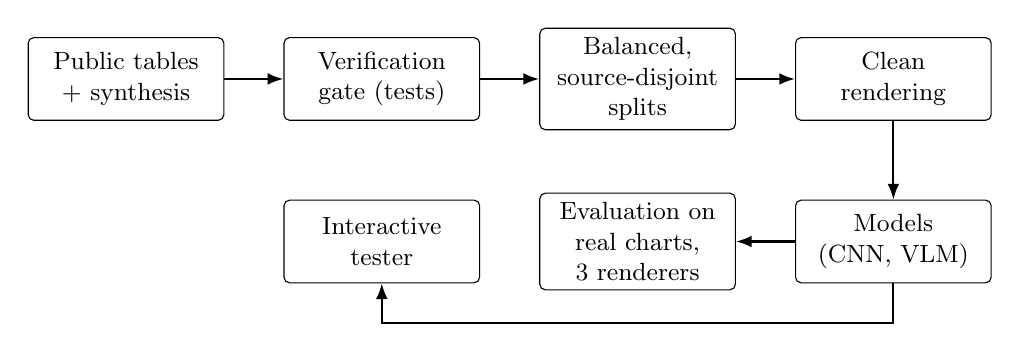
\begin{tikzpicture}[
  node distance=0.55cm and 0.75cm,
  box/.style={draw,rounded corners=2pt,align=center,minimum height=1.05cm,
              text width=2.25cm,font=\small},
  ar/.style={-{Latex[length=2mm]},thick}]
\node[box] (a) {Public tables\\+ synthesis};
\node[box,right=of a] (b) {Verification\\gate (tests)};
\node[box,right=of b] (c) {Balanced,\\source-disjoint\\splits};
\node[box,right=of c] (d) {Clean\\rendering};
\node[box,below=1.0cm of d] (e) {Models\\(CNN, VLM)};
\node[box,left=of e] (f) {Evaluation on\\real charts,\\3 renderers};
\node[box,left=of f] (g) {Interactive\\tester};
\draw[ar] (a)--(b); \draw[ar] (b)--(c); \draw[ar] (c)--(d);
\draw[ar] (d)--(e); \draw[ar] (e)--(f); \draw[ar] (e.south) |- ++(0,-0.5) -| (g.south);
\end{tikzpicture}
\caption{Pipeline: tables are admitted only through the verification gate, split by
source, rendered without label-dependent marks, used to train models, and evaluated
on real charts drawn by three plotting libraries.}
\label{fig:pipeline}
\end{figure}

\section{Data: InsightVLM-20K}
\label{sec:data}

\subsection{Task Definition}

\textbf{Input:} a chart image. \textbf{Output:} the statistical finding the chart
shows (one of 20 classes). Every sample additionally carries the data table, the
statistics that support the finding, a reasoning chain and an evidence-grounded
insight, so the same corpus supports table reconstruction, generation and grounding.

\subsection{Label Space}

Twenty finding classes span four analysis families. Each class was admitted only
if it is (i) verifiable by a standard named statistical test, (ii) mutually
exclusive from every other class by explicit guard conditions, and (iii) visible
in a rendered chart.

\begin{table}[h]\centering\small
\caption{Finding families and their classes.}
\label{tab:families}
\begin{tabular}{llp{7.1cm}}
\toprule
\textbf{Family} & \textbf{$n$} & \textbf{Classes} \\
\midrule
Distribution & 6 & normal, right-skew, left-skew, bimodal, heavy-tail, uniform \\
Relationship & 6 & strong positive, strong negative, none, non-linear monotonic,
                  non-linear non-monotonic, heteroscedastic \\
Temporal & 5 & increasing, decreasing, seasonal, changepoint, anomaly spike \\
Group & 3 & significant difference, no difference, dominant category \\
\bottomrule
\end{tabular}
\end{table}

\subsection{The Verification Gate}
\label{sec:gate}

This is the methodological core of the thesis and the mechanism by which
Gap~G1 (Section~\ref{sec:ourgap}) is closed. \textbf{A label is never asserted;
it is tested.} Three rules govern construction.

\paragraph{Rule 1 --- subsample before verifying.} Data is reduced to its final
plotted size \emph{before} the statistical test runs. Verifying a parent
dataframe and then plotting a subsample would produce ground truth describing
data the image does not show.

\paragraph{Rule 2 --- exactly one class must match.} A candidate satisfying two
classes' guards is discarded as ambiguous rather than multi-labelled. This keeps
the primary label single-valued and the confusion matrix interpretable, at the
cost of excluding compound findings (see Section~\ref{sec:risks}).

\paragraph{Rule 3 --- rejection is free; wrong labels are not.} Every guard drops
a sample rather than mislabelling it. More candidates can always be mined; a
poisoned label cannot be undone.

\paragraph{Why robust statistics are mandatory.} A naive implementation of these
tests fails in ways we measured, and three guards exist specifically to prevent
it:

\begin{itemize}[leftmargin=1.3em]
  \item \emph{Moment skewness is not tail-robust.} Over 40 draws of a symmetric
  Student-$t(4)$ sample, the moment estimator alone mislabelled $12.5\%$ as
  skewed. Requiring agreement with Bowley (quartile) skewness eliminated this.
  \item \emph{Hartigan's dip test is calibrated against the uniform}, so a
  genuinely flat distribution trips $p<0.05$ roughly $5\%$ of the time. The
  bimodal guard therefore additionally requires a KS test against the uniform to
  reject.
  \item \emph{A monotone ramp defeats changepoint detection}, producing a
  high-SNR ``changepoint''. The guard therefore requires a two-level step model to
  beat a linear fit \emph{and} an abruptness ratio $>0.55$ (measured: true step
  $1.15$, smooth rise-then-fall $0.18$, pure ramp $0.14$).
\end{itemize}

Generator-to-class fidelity over 10 seeds $\times$ 20 classes is $95.5\%$; every
remaining miss is a conservative rejection, never a wrong label.

\subsection{Two Construction Tracks}

A balanced corpus cannot be built from real data alone. Public repositories hold
thousands of right-skewed columns and almost no clean inverted-U relationships:
mining 719 real tables yielded exactly \textbf{ten}. The dataset is therefore a
declared hybrid, and we state the mix rather than obscuring it.

\emph{Track R (real-seeded)} mines every plottable view from 719 public tables
(OpenML, World Bank, Our World in Data, vega-datasets, seaborn-data, UCI).
\emph{Track S (controlled synthesis)} generates data whose property holds by
construction, from a domain vocabulary spanning health, economics, environment,
engineering, education and retail. \textbf{Both tracks pass the identical gate.}

Provenance is balanced \emph{within} each class rather than real-first;
real-first would leave some classes almost entirely real and others almost
entirely synthetic, letting a model key on provenance instead of the statistical
pattern.

\subsection{Splits and the Supplementary Real Pool}
\label{sec:splits}

Splits are $14{,}000/2{,}000/4{,}000$, exactly $700/100/200$ per class, and
\textbf{source-disjoint} for real data: a hash of the source-table identifier
assigns every chart derived from one table to a single split. The real subsets hold
$4{,}338$ training, $553$ validation and $1{,}192$ test charts; real class frequencies
are uneven because public data are.

Balance caps real data at 500 per class, so the gate admitted more real charts than
the balanced splits use. We keep the surplus as a \textbf{supplementary real training
pool}: candidates whose source table the same hash assigns to \emph{train}, with exact
duplicates of any dataset sample removed and at most 400 per class. The build asserts
that no validation or test source contributes. The pool adds $2{,}545$ real training
charts in nine classes, raising real training data from $4{,}338$ to $6{,}883$.

\begin{table}[h]\centering\small
\caption{Dataset summary and integrity audit.}
\label{tab:dataset}
\begin{tabular}{lr}
\toprule
Samples & $20{,}000$ \\
Classes & 20, exactly $1{,}000$ each \\
Chart types & 26 \\
Provenance & $6{,}083$ real (654 source tables) / $13{,}917$ synthetic \\
Supplementary real training pool & $2{,}545$ (train-split sources only) \\
Underlying data points & $8{,}487{,}134$ \\
\midrule
Label re-verification from stored data & $100.00\%$ \\
Leaked sources across splits & 0 of 654 \\
Duplicate data fingerprints & 0 \\
Real test charts with near-duplicate data in training (Sec.~\ref{sec:rq5}) & 85 of 1{,}192 \\
Grounding boxes outside canvas & 0 \\
\bottomrule
\end{tabular}
\end{table}

\section{Rendering}
\label{sec:render}

Charts are drawn with matplotlib and seaborn on a fixed $768\times576$ canvas across
26 chart types and 8 visual styles. Each sample's style is chosen from a CRC32 hash of
its identifier, so rendering is reproducible across processes.\footnote{The first
version used Python's built-in \texttt{hash()}, which is salted per process, so styles
could not be reproduced. This was corrected in version 2.} Grounding boxes marking the
evidence (outlier band, modal bin, change point, anomalous points, dominant wedge) are
emitted in image pixel coordinates. Tight bounding-box cropping is deliberately
disabled: it resizes the canvas \emph{after} the axes transform is read, silently
invalidating every box. Dates stored as epoch timestamps are plotted as calendar dates.

\subsection{No Label-Dependent Marks (Version 2)}
\label{sec:v2}

The first release drew annotations on time-series charts that depended on the label:
a fitted trend line only on increasing and decreasing series, a vertical line at the
change point only on level-shift series, and circles only around anomalies. The
seasonal class carried no mark, so the absence of a mark was itself informative. Such
marks let a model identify the class without reading the data. Version 2 draws no
label-dependent marks; the evidence survives only as grounding boxes in the metadata.
No other family drew label-dependent marks (regression lines on scatter plots are drawn
independently of the label). Chapter~\ref{ch:results} measures how strongly models had
exploited the marks. All results in this thesis use version 2.

\subsection{Cross-Renderer Test Sets}

All training charts come from one plotting library, so a model could learn
matplotlib's appearance rather than the statistics. The 1{,}192 real test tables were
therefore re-drawn by two more libraries from the same stored data:
\emph{Plotly}, with five templates (excluding the one that imitates seaborn), and
\emph{Vega-Lite}, with nine themes (excluding those that match a matplotlib training
style). Chart types map to each library's nearest native form; where none exists the
substitute is a form the taxonomy lists as valid for every class that chart type can
carry, so no label becomes unreadable.

\subsection{Training-Only Renderer Augmentation}

Every training and supplementary chart was also rendered twice more, for training
only: by Plotly, and by matplotlib with randomised fonts, font sizes, line and marker
sizes, colours, background tints, gridlines, spines and title placement. The data and
chart type are unchanged, so the label is too. No validation or test chart is rendered
this way and no Vega-Lite render is used in training, so \textbf{Vega-Lite remains a
renderer that no model has seen}, and the Plotly test set becomes a seen-renderer test
for augmented models.

\section{Evaluation Protocol}
\label{sec:protocol}

This section addresses RQ5 and objective O6.

\subsection{Why the Conventional Baseline Is Wrong Here}

With 20 balanced classes, chance is $5\%$. But chart type is associated with the
finding \emph{by construction} --- a pie chart can only carry a composition
finding, a QQ plot only a distribution finding. A model consulting \emph{no pixels
at all}, predicting the most common class for each chart type, reaches
$\mathbf{0.288}$. Reporting against $5\%$ would credit a model with roughly 24
points it did not earn. We therefore use the chart-type prior as the floor.

\subsection{A Data Oracle Gives the Ceiling}

Running the verification battery on each sample's stored data table --- seeing the
numbers, not the picture --- yields $\mathbf{0.9995}$. This is the deterministic
rule-based pipeline of RQ2/O3, and a vision model is interesting only within
$[0.288,\ 0.9995]$.

\subsection{Real Charts Are the Headline}

Because the corpus is majority synthetic, mixed-test accuracy cannot distinguish
learning the statistics from learning the generator. The headline metric is accuracy
on the $1{,}192$ real test charts (RQ4/O5), reported for the matplotlib render and for
the Plotly and Vega-Lite re-renders. Every accuracy carries a 95\% bootstrap confidence
interval (4{,}000 resamples), and differences between systems scored on the same
charts are tested with exact McNemar tests. \textbf{Every choice of model, checkpoint,
ensemble member and hyperparameter is made on the validation split}; the test split is
scored once.

\subsection{Shortcut and Bias Audit}

Eleven failure modes are measured against thresholds fixed in advance
(Table~\ref{tab:bias}). All pass on version 2.

\begin{table}[h]\centering\small
\caption{Shortcut and bias audit on version 2; all eleven tests pass.}
\label{tab:bias}
\begin{tabular}{lrr}
\toprule
\textbf{Test} & \textbf{Value} & \textbf{Threshold} \\
\midrule
Class balance (imbalance ratio) & 1.000 & $=1.000$ \\
Split balance (max s.d.) & 0.0000 & $<0.01$ \\
Chart type $\rightarrow$ label (pixel-free prior) & 0.2883 & reported as floor \\
Render style $\rightarrow$ label (Cram\'er's $V$) & 0.0000 & $<0.05$ \\
\textbf{Provenance detectability (AUC)} & \textbf{0.551} & $<0.75$ \\
Axis-text shortcut (macro-F1) & 0.3688 & $<0.55$ \\
Pixel-statistic shortcut (macro-F1) & 0.4038 & $<0.55$ \\
Source concentration (top share) & 17.2\% & $<35\%$ \\
Length confound (within family) & 2.04 & $<4.0$ \\
Subject-domain balance & 22.8\% & $<45\%$ \\
Category-vocabulary spread & 13.0\% & $<35\%$ \\
\bottomrule
\end{tabular}
\end{table}

Provenance detectability matters most: with $69.6\%$ of samples synthetic, the obvious
objection is that a model learns to recognise generated charts. A classifier on
low-level pixel statistics separates real from synthetic at $\mathrm{AUC}=0.551$ ---
close to chance. The audit examines metadata and pixel statistics, however, not what a
trained model attends to; it did \emph{not} detect the version-1 marks
(Section~\ref{sec:v2}), which were found by inspecting the renderer. We therefore added a
direct ablation (Section~\ref{sec:leak}).

\section{Models}
\label{sec:models}

\subsection{Discriminative Models (O2)}

ImageNet-pretrained ResNet-101, ResNet-50 and DenseNet-121 are fine-tuned at
$384\times384$ for up to 12 epochs with AdamW (learning rate $3\times10^{-4}$,
weight decay 0.05), a one-cycle schedule, label smoothing 0.1 and mixed precision on
two T4 GPUs. Two choices target real-chart accuracy directly:
\begin{itemize}[leftmargin=1.3em]
  \item \textbf{Real-data oversampling.} A weighted sampler draws about half of every
  batch from real charts (31\% of the balanced training split is real).
  \item \textbf{Real-validation checkpointing.} The checkpoint kept is the epoch with
  the highest accuracy on the 553 \emph{real} validation charts, with mixed validation
  accuracy as the tie-break. Mixed accuracy saturates near 0.95 and says little.
\end{itemize}
Models are trained in three steps, each an ablation of the next: on the balanced split;
with the supplementary real pool added; and with renderer augmentation added (each
epoch shows each training chart as one of its three renders, uniformly).

\paragraph{Augmentation constraint.} Horizontal and vertical flips are
\emph{excluded}. Mirroring a scatter converts a strong positive correlation into
a strong negative one, and mirroring a line chart converts an increasing trend
into a decreasing one --- both separate classes here, so the default augmentation
would silently corrupt roughly $30\%$ of labels. Only label-preserving transforms
(mild crop and scale, colour jitter, blur, small erasures) are used.

\paragraph{Ensemble.} The deployed model averages the class probabilities of the
full-recipe members (supplementary pool and renderer augmentation) with equal weights.
Probabilities are averaged rather than logits, whose scales differ across
architectures. A label-shift correction towards real-data class frequencies, estimated
from training data only, is available with its strength tuned on validation (it is
not used: the tuned strength is zero). Greedy ensemble selection on validation and the
average of all trained models are reported as alternatives.

\subsection{Zero-Shot Vision--Language Models}

To test whether current general-purpose VLMs can already do the task, Qwen2.5-VL-3B,
Qwen2.5-VL-7B and Qwen3-VL-8B receive each real test chart with all 20 class names and
one-line definitions and must answer with one class name (greedy decoding, no task
training). Answers are parsed by exact label match; over 99.9\% parse.

\subsection{Generative Model: InsightVLM (O2, O3)}

Qwen2-VL-2B adapted with QLoRA ($r=16$, 4-bit NF4, $18.5$M trainable parameters,
$0.83\%$ of the model), trained one epoch on $4{,}000$ samples. The supervision
target is the reasoning chain plus the insight, so the model learns to produce
evidence-grounded prose rather than a class identifier. Numeric fidelity is the share
of numbers the model cites that match the ground-truth statistics to two decimals.
This model was trained and evaluated on version-1 renders before the leak was found;
Chapter~\ref{ch:results} reports it with that caveat.

\subsection{Evidence-Grounding Evaluation (O4)}

For each real test chart that carries at least one evidence box, the Grad-CAM map of
each deployed member for its predicted class is computed at the last convolutional
block, upsampled, and its peak mapped back to image pixels. A \emph{hit} is a peak
inside any evidence box. The control is a uniformly random point inside the plot area,
whose expected hit rate equals the evidence boxes' share of the plot area, so large
evidence regions cannot inflate the result.

\subsection{Interactive Tester}

A Gradio web application (Appendix~\ref{app:tester}) loads the deployed ensemble and
runs uploaded charts through exactly the pipeline that was scored. It reports the
finding, its confidence, how many members agree, and the statistical test that defines
the class, and can draw random held-out test charts to show predictions against the
verified ground truth.

\section{What Could Go Wrong}
\label{sec:risks}

\begin{description}[leftmargin=1.4cm,style=nextline,font=\bfseries]
  \item[R1. Synthetic majority.] $69.6\%$ of samples are synthetic; balance forced
  this. \emph{Mitigation:} provenance balanced within each class, identical gate
  for both tracks, real charts reported as the headline, and a supplementary real pool
  for training. \emph{Residual risk:} the real subset may not represent real charts
  broadly.

  \item[R2. Single-label design.] Compound findings were excluded, not handled, so
  the model will not learn to report a trend and an anomaly together.
  \emph{Mitigation:} stated as a limitation; multi-label extension is future work.

  \item[R3. Difficulty axis does not track difficulty.] Accuracy does not follow
  the evidence-margin tertiles (Spearman $0.034$). Extreme margins produce
  degenerate charts --- a residual spread ratio of $1537$ renders as a single
  vertical smear. \emph{Mitigation:} reported as a finding about chart benchmarks
  rather than presented as a working difficulty axis.

  \item[R4. Renderer monoculture.] Training charts come from one plotting library.
  \emph{Mitigation:} Plotly and Vega-Lite test sets measure the effect, and
  training-only renderer augmentation reduces it; Vega-Lite is held out entirely.

  \item[R5. Thresholds are conventions.] $|r|>0.7$ as ``strong'' and
  $\varepsilon^2>0.14$ as ``large'' are choices. \emph{Mitigation:} all cuts are
  recorded explicitly so results can be re-derived under alternatives.

  \item[R6. Template recitation by the VLM.] The training target embeds each class
  description verbatim, so the model could score well by memorising a phrase.
  \emph{Mitigation:} the real/synthetic gap is the diagnostic --- observed
  $0.683$ vs $0.844$, comparable in magnitude to the CNNs, indicating chart
  reading rather than recitation.

  \item[R7. Compute constraints.] Training ran on free Kaggle T4 GPUs with a weekly
  quota; the generative result used $4{,}000$ samples, one epoch and 2B parameters at
  4-bit. \emph{Mitigation:} reported as a compute-constrained floor, not a ceiling.

  \item[R8. Rendering leaks.] A renderer can reveal the label without the audit
  noticing. This happened (Section~\ref{sec:v2}). \emph{Mitigation:} version 2 removes
  every label-dependent mark, and a with/without ablation quantifies the effect.

  \item[R9. Selection on the test set.] An earlier ensemble was chosen by ranking
  combinations on test accuracy, which inflates the reported number.
  \emph{Mitigation:} all selection now uses validation only (Section~\ref{sec:protocol}).
\end{description}

\section{Reproducibility}

The corpus rebuilds end to end with \texttt{run\_all.py}; \texttt{07\_validate.py}
(integrity) and \texttt{10\_bias\_audit.py} (shortcuts) audit it. The clean renders,
the supplementary pool, the Plotly and Vega-Lite renders and the augmentation renders
are produced by \texttt{06\_render.py}, \texttt{12\_extra\_real.py},
\texttt{11\_render\_plotly.py} and \texttt{13\_render\_vega.py}. Training notebooks are
generated by \texttt{train/make\_split\_notebooks.py}, and every reported number comes
from \texttt{final\_ensemble.py}, \texttt{stats\_report.py},
\texttt{grounding\_eval.py} and \texttt{ablate\_marks.py}. All thresholds live in a
single module so results can be re-derived under alternative conventions.
Documentation follows the datasheet standard of \citet{datasheets}.
       % Week 3: data, methods, protocol, risks
\chapter{Results}
\label{ch:results}

This chapter reports every result on the held-out test split, scored once, with
selection done on validation only (Section~\ref{sec:protocol}). It begins with a
correction to results reported in earlier drafts, because every later number depends
on it, and then answers the five research questions in turn.

\section{A Correction: Two Problems in the Earlier Results}
\label{sec:leak}

Earlier drafts of this work (Chapter~\ref{ch:method}, version~1) reported an ensemble
reaching $0.865$ on real test charts. That number had two problems.

\paragraph{Selection on the test set.} The ensemble was chosen by ranking every
combination of trained models on test accuracy. Selecting the same models on
validation instead gives $0.845$. The difference is small, but a number chosen on the
test set is not a test result.

\paragraph{A rendering leak.} Version-1 time-series charts carried marks that depended
on the label (Section~\ref{sec:v2}). To measure how much the models relied on them, the
same 1{,}000 test time series were rendered twice with identical styles, once with the
marks and once without, and scored with two ResNets trained on version 1
(Table~\ref{tab:leak}, Figure~\ref{fig:leak}).

\begin{table}[h]\centering\small
\caption{Accuracy of version-1 models on test time series rendered with and without the
label-dependent marks. Only the marks differ between the two renders.}
\label{tab:leak}
\begin{tabular}{lcccc}
\toprule
& \multicolumn{2}{c}{\textbf{ResNet-101}} & \multicolumn{2}{c}{\textbf{ResNet-50}} \\
\cmidrule(lr){2-3}\cmidrule(lr){4-5}
\textbf{Test charts} & with marks & without & with marks & without \\
\midrule
Real time series ($n=305$)       & 0.957 & \textbf{0.311} & 0.944 & \textbf{0.407} \\
Synthetic time series ($n=695$)  & 1.000 & 0.801 & 1.000 & 0.911 \\
\quad level shift                & 1.000 & 0.355 & 1.000 & 0.705 \\
\quad increasing                 & 0.975 & 0.570 & 0.930 & 0.570 \\
\quad seasonal (never marked)    & 0.970 & 0.970 & 0.990 & 0.990 \\
\bottomrule
\end{tabular}
\end{table}

\begin{figure}[h]\centering
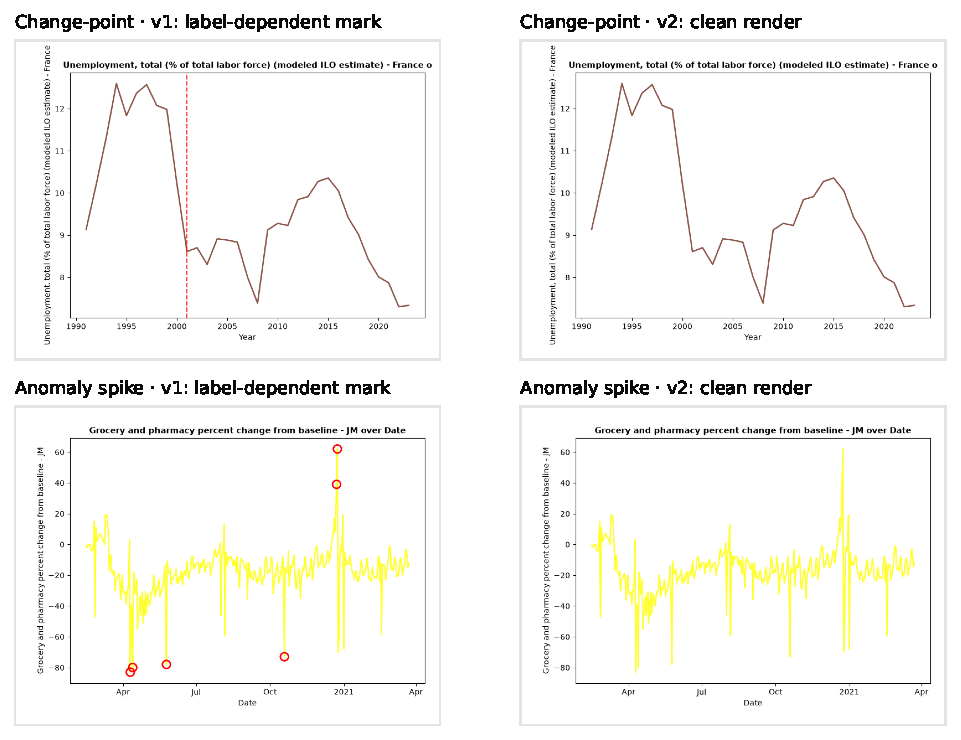
\includegraphics[width=\linewidth]{fig_marks_examples.pdf}\\[0.5em]
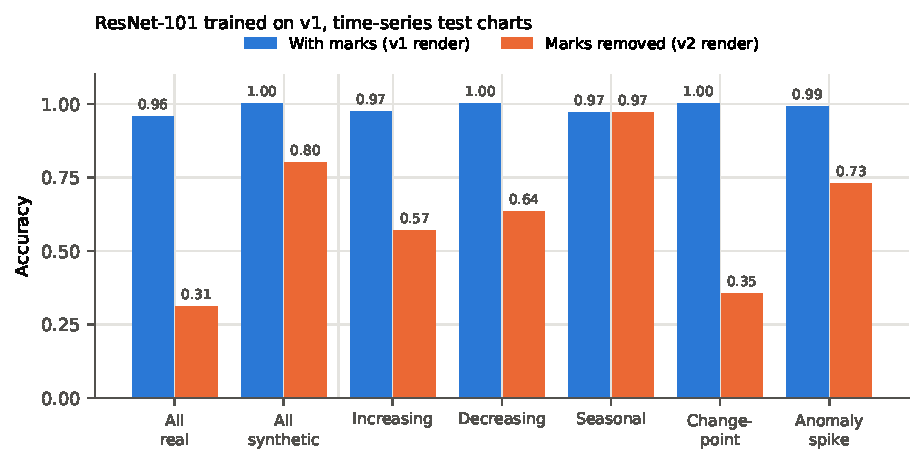
\includegraphics[width=\linewidth]{fig_marks_ablation.pdf}
\caption{Top: the same real data rendered with a version-1 label-dependent mark and in
the released version-2 form. Bottom: accuracy of a version-1 ResNet-101 with and
without the marks.}
\label{fig:leak}
\end{figure}

Without the marks, accuracy on real time series fell from $0.957$ to $0.311$: the
models had largely learned to read the annotation rather than the data. The seasonal
class, the only temporal class that never carried a mark, was unaffected, which isolates
the cause. The zero-shot vision--language models of Section~\ref{sec:rq1}, which never
saw version-1 training data, changed by only 1--2.5 points on all real charts and
4--10 points on real time series. This is shortcut learning~\citep{geirhos} of the
plainest kind, and the shortcut audit (Table~\ref{tab:bias}) did not detect it, because
the audit examines metadata and pixel statistics rather than what a trained model
relies on.

\textbf{Every result from here on uses version 2, trains new models on it, and selects
on validation only.}

\section{RQ1: Can a Model Identify the Finding from the Chart Alone?}
\label{sec:rq1}

Table~\ref{tab:main} gives the main results and Figure~\ref{fig:main} the comparison.
The deployed ensemble (the equal-weight average of the two full-recipe models) reaches
\textbf{0.867} on the 1{,}192 real test charts (95\% CI $[0.846, 0.886]$) and
\textbf{0.999} on synthetic ones, $0.959$ over all 4{,}000 test charts. Macro-F1 on
real charts is $0.776$, lower than accuracy because the rarest real classes are also
the hardest.

\begin{table}[h]\centering\small
\caption{Accuracy on the 1{,}192 real test charts drawn by three plotting libraries,
and on synthetic test charts. Brackets: 95\% bootstrap CI. $^\dagger$Fixed 400-chart
synthetic sample.}
\label{tab:main}
\resizebox{\linewidth}{!}{%
\begin{tabular}{lcccc}
\toprule
 & \multicolumn{3}{c}{\textbf{Real test charts}} & \\
\cmidrule(lr){2-4}
\textbf{System} & \textbf{matplotlib} & \textbf{Plotly} & \textbf{Vega-Lite} & \textbf{Synthetic} \\
\midrule
Chart-type prior (no pixels)            & \multicolumn{4}{c}{0.288 (all test charts)} \\
Qwen2.5-VL-3B, zero-shot                & 0.306 [0.281, 0.332] & -- & -- & 0.303$^\dagger$ \\
Qwen2.5-VL-7B, zero-shot                & 0.411 [0.383, 0.440] & -- & -- & 0.498$^\dagger$ \\
Qwen3-VL-8B, zero-shot                  & 0.468 [0.439, 0.496] & -- & -- & 0.648$^\dagger$ \\
\midrule
ResNet-101, balanced split              & 0.841 & 0.747 & 0.607 & 0.997 \\
ResNet-50, balanced split               & 0.828 & 0.722 & 0.608 & 0.998 \\
ResNet-101, + supplementary pool        & 0.840 & 0.735 & 0.602 & 0.999 \\
ResNet-50, + supplementary pool         & 0.845 & 0.760 & 0.599 & 0.998 \\
DenseNet-121, + supplementary pool      & 0.861 & 0.771 & 0.638 & 0.997 \\
ResNet-101, + pool + renderer aug.      & 0.859 & 0.854 & 0.650 & 0.998 \\
DenseNet-121, + pool + renderer aug.    & 0.855 & 0.852 & 0.712 & 0.998 \\
\textbf{Ensemble (two full-recipe models)} & \textbf{0.867} [0.846, 0.886] & \textbf{0.857} [0.836, 0.877] & \textbf{0.716} [0.690, 0.741] & \textbf{0.999} \\
\midrule
Statistical oracle on the data table    & \multicolumn{4}{c}{0.9995 (all test charts)} \\
\bottomrule
\end{tabular}}
\end{table}

\begin{figure}[h]\centering
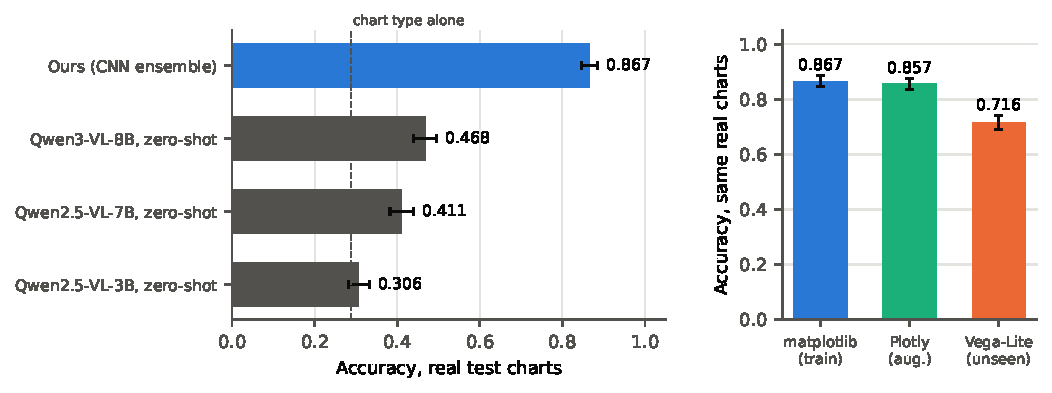
\includegraphics[width=\linewidth]{fig_results.pdf}
\caption{Left: accuracy on the real test charts (matplotlib renders) with 95\% bootstrap
CIs; the dashed line is the chart-type prior. Right: the deployed ensemble on the same
real charts drawn by the training renderer, by Plotly (used only as training
augmentation) and by Vega-Lite (never seen).}
\label{fig:main}
\end{figure}

\paragraph{Zero-shot vision--language models cannot do this task reliably.} The best,
Qwen3-VL-8B, reaches 0.468; the smallest, Qwen2.5-VL-3B, is barely above the 0.288
floor that uses no pixels at all. The ensemble is right on 511 charts where Qwen3-VL-8B
is wrong and wrong on only 36 where it is right (exact McNemar $p<10^{-100}$; the same
holds for the other two models). Naming a statistical finding from a chart is therefore
not a capability current general-purpose VLMs already have.

\paragraph{How the result was built.} Each step in Table~\ref{tab:main} changes one
thing. Adding the supplementary real pool helped ResNet-50 (+1.7 points) but not
ResNet-101 ($-0.1$); DenseNet-121 trained on the pool was the strongest single model on
matplotlib charts ($0.861$). Renderer augmentation raised ResNet-101 from $0.840$ to
$0.859$ and, as the next section shows, mattered far more on other renderers. Choosing
the ensemble differently changes little: averaging all seven trained models gives
$0.862$, greedy selection on validation $0.865$.

\paragraph{Where the model fails.} Figures~\ref{fig:conf} and~\ref{fig:perclass} break
the result down. Errors stay almost entirely within a family, and the family with the
most errors is distribution shape ($0.763$ on real charts, against $0.886$--$0.930$ for
the others). The commonest confusions are between classes that differ in degree rather
than kind: bimodal read as right-skewed (19 of 100), heavy-tailed read as right-skewed
(13 of 26) and significant group differences read as none (12 of 100). Accuracy is
lowest where real examples are rare: heavy tails ($0.385$, $n=26$), seasonality
($0.462$, $n=13$), left skew ($0.474$, $n=19$), and the inverted-U relationship, of
which only two real test charts exist.

\begin{figure}[h]\centering
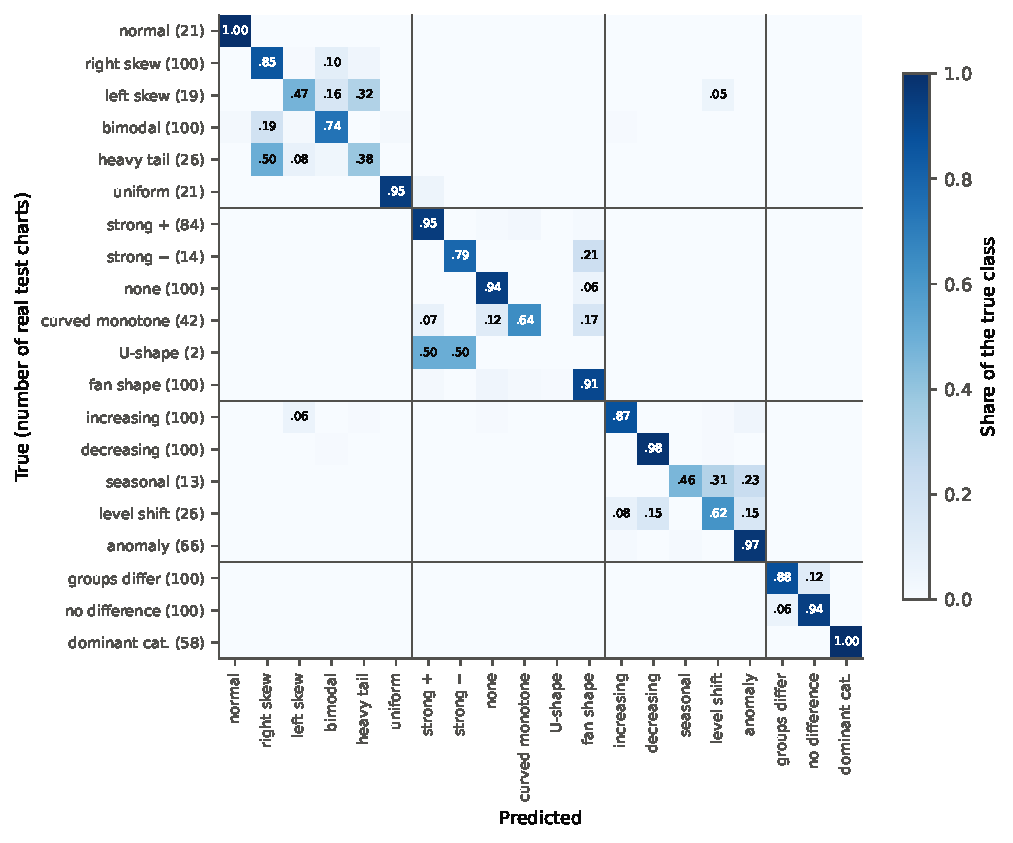
\includegraphics[width=0.92\linewidth]{fig_confusion.pdf}
\caption{Confusion matrix of the deployed ensemble on the 1{,}192 real test charts,
normalised by true class; lines separate the four families. The number of real charts
per class is in brackets.}
\label{fig:conf}
\end{figure}

\begin{figure}[h]\centering
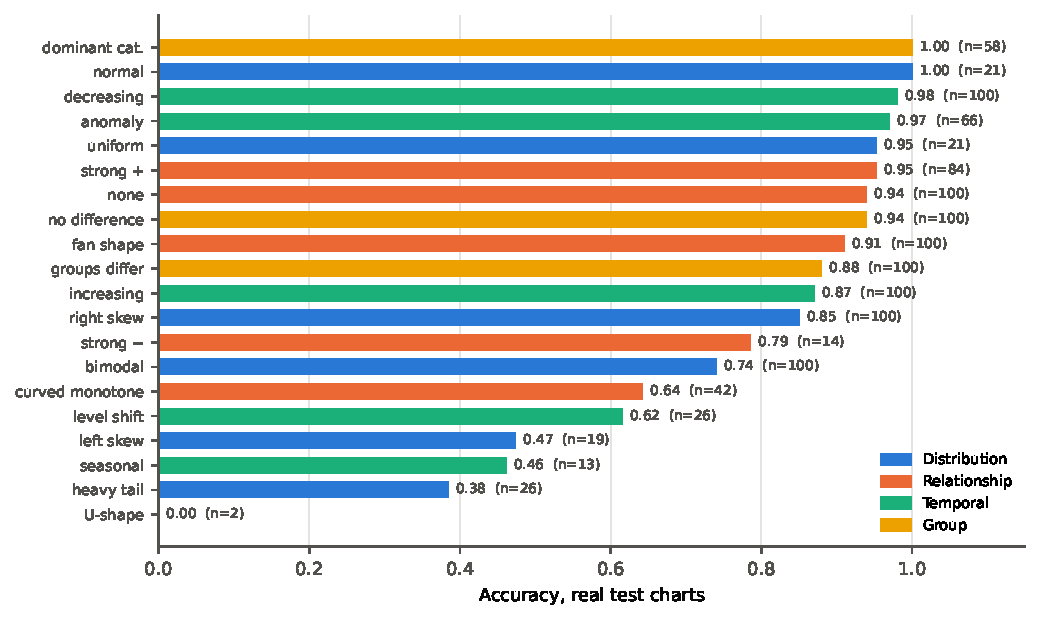
\includegraphics[width=\linewidth]{fig_per_class.pdf}
\caption{Accuracy of the deployed ensemble per class on the real test charts.}
\label{fig:perclass}
\end{figure}

\paragraph{Answer to RQ1.} Yes, for most findings. A fine-tuned vision model names the
statistical finding of a real chart correctly 86.7\% of the time without being asked a
question, far above both the pixel-free floor and current zero-shot VLMs. It remains
unreliable for subtle distribution shapes and for classes with little real data.

\section{RQ2: Model Insights versus a Deterministic Statistical Pipeline}
\label{sec:rq2}

The deterministic pipeline is the verification battery run on the chart's stored data
table. It recovers the finding for 0.9995 of test charts, and the two exceptions lie
within 1\% of a guard threshold and fall to \emph{no class} rather than to a wrong one.
Its numbers are exact by construction.

The generative model (Qwen2-VL-2B with QLoRA, Section~\ref{sec:models}) was evaluated on
a 300-chart test subset. It named the correct finding for $0.800$ of charts ($0.683$ on
real, $0.844$ on synthetic), but \textbf{only 13.8\% of the numbers it cited matched the
ground-truth statistics}. It has learned the vocabulary and structure of statistical
reasoning while largely inventing the supporting numbers. This model was trained and
scored on version-1 renders; its class accuracy on time series may be inflated by the
leak, but numeric fidelity concerns the numbers in its text and is not affected by marks.

\paragraph{Answer to RQ2.} Far below. The rule-based pipeline is essentially always right
and exact; the generative model is right about the finding four times in five but cites
correct numbers about one time in seven. Fluent statistical language is much easier to
produce than true statistical language, and only a dataset with verified statistics can
tell them apart.

\section{RQ3: Is the Model Looking at the Evidence?}
\label{sec:rq3}

We tested whether the deployed models attend to the evidence that licenses a label,
using the pointing game of Section~\ref{sec:models}: for each of the 1{,}023 real test
charts that carry at least one evidence box, a hit is a Grad-CAM peak inside an evidence
box, and the control is a random point in the plot area (Table~\ref{tab:grounding}).

\begin{table}[h]\centering\small
\caption{Pointing game on 1{,}023 real test charts. \emph{Gain} is the pointing rate
minus the random-point control, with a 95\% bootstrap CI.}
\label{tab:grounding}
\begin{tabular}{lccc}
\toprule
\textbf{Charts} & \textbf{Pointing} & \textbf{Random control} & \textbf{Gain [95\% CI]} \\
\midrule
Temporal ($n=305$)      & 0.649 & 0.495 & $+0.154$ [$+0.139$, $+0.168$] \\
Group ($n=258$)         & 0.599 & 0.489 & $+0.110$ [$+0.064$, $+0.153$] \\
Relationship ($n=173$)  & 0.642 & 0.569 & $+0.073$ [$+0.029$, $+0.115$] \\
Distribution ($n=287$)  & 0.253 & 0.254 & $-0.002$ [$-0.035$, $+0.033$] \\
\midrule
ResNet-101 member       & 0.543 & 0.439 & $+0.105$ [$+0.081$, $+0.130$] \\
DenseNet-121 member     & 0.504 & 0.439 & $+0.066$ [$+0.042$, $+0.089$] \\
\textbf{All}            & \textbf{0.524} & \textbf{0.439} & $\mathbf{+0.085}$ [$+0.068$, $+0.102$] \\
\bottomrule
\end{tabular}
\end{table}

The models point at the evidence more often than chance overall ($+8.5$ points), most
clearly for time series ($+15.4$) and group comparisons ($+11.0$), less for relationships
($+7.3$), and \emph{not at all} for distributions ($-0.2$, CI spanning zero). Pointing is
slightly better when the prediction is correct (0.570 and 0.533 for the two members).

Two readings are possible for the distribution family, and the data cannot yet separate
them. A distribution's shape is a property of the whole histogram or density rather than
of one region, so an evidence box around the modal bin or the outlier band may simply be
the wrong reference for where a model should look. Alternatively, the models may judge
shape from global cues. Either way, distribution is also the family with the lowest
accuracy (0.763), so weak grounding and weak accuracy coincide.

\paragraph{Answer to RQ3.} Partly. The model's attention is tied to the verified evidence
beyond chance for three of four families, but only modestly: about half of all peaks fall
inside an evidence box, against 44\% for a random point. The CNN classifiers are not
generating insights, so this measures whether their decisions rest on the evidence, not
whether a generated sentence is traceable; the generative model's traceability is limited
by its 13.8\% numeric fidelity (Section~\ref{sec:rq2}).

\section{RQ4: Generalisation to Real-World Charts}
\label{sec:rq4}

Real-world generalisation has two parts: real \emph{data}, and charts drawn by
\emph{other tools}.

\paragraph{Real data.} On matplotlib charts the gap between synthetic and real test
charts is 13.2 points ($0.999$ against $0.867$). Real charts are harder: 44\% of real
samples fall in the hardest evidence-margin tertile against 29\% of synthetic ones, and
real data are noisier and less clean-cut than generated data.

\paragraph{Other plotting libraries.} Trained on matplotlib alone, every model loses
8.5--10.6 points when the same real data is drawn by Plotly and 22--25 points when it
is drawn by Vega-Lite (Table~\ref{tab:main}). The models had learned part of matplotlib's
appearance. Training-only renderer augmentation (Plotly renders plus randomised
matplotlib styles) closes most of the Plotly gap, as expected for a renderer seen in
training, and, more tellingly, lifts accuracy on Vega-Lite, \textbf{which no model has
seen}, from $0.60$--$0.64$ to $0.65$--$0.71$, without costing matplotlib accuracy. The
deployed ensemble reaches $0.857$ on Plotly and $0.716$ on Vega-Lite.

\paragraph{Answer to RQ4.} A model trained on a mostly synthetic corpus generalises to
real data well (0.867) when the chart is drawn the way its training charts were, and
reasonably (0.716) when it is drawn by a tool it has never seen. The 15-point
unseen-renderer gap is the main open problem this dataset exposes, and renderer
diversity in training is the most effective remedy we found.

\section{RQ5: Evaluation Protocol and Shortcuts}
\label{sec:rq5}

The protocol of Section~\ref{sec:protocol} changed the conclusions in three ways.

\begin{enumerate}[leftmargin=1.4em]
  \item \textbf{The floor.} A rule using no pixels reaches 0.288, not 0.05. The weakest
  zero-shot model (0.306) is barely above it, which a 5\% baseline would have hidden.
  \item \textbf{Real charts as the headline, three renderers.} Mixed accuracy ($0.959$)
  hides a 13-point real/synthetic gap and a 15-point unseen-renderer gap, both of which
  are the numbers that matter for use.
  \item \textbf{Selection on validation only.} Selecting on test inflated the earlier
  result by two points; selection on 553 real validation charts is itself noisy, so the
  deployed ensemble uses equal weights and the alternatives are reported.
\end{enumerate}

The eleven-test shortcut audit passes on version 2 (Table~\ref{tab:bias}); in
particular, pixel statistics cannot tell real from synthetic charts (AUC 0.551). But the
audit missed the rendering leak of Section~\ref{sec:leak}: an audit of data and pixels
does not replace testing what a trained model uses.

\paragraph{Answer to RQ5.} Report accuracy on real charts, drawn by more than one
renderer, against a pixel-free floor and a data-oracle ceiling, with confidence
intervals, paired tests and validation-only selection; and test trained models directly
for shortcuts, because a data audit alone did not catch the one that mattered.

\section{Human Baseline}
\label{sec:human}

A human baseline was designed and deployed: a web form showing 200 real test charts
(10 per class; 2 for the inverted-U class) with the 20 findings in plain language, in a
different random order for each annotator, with anonymous chart identifiers and no
annotator able to see another's answers. At the time of writing one complete submission
had been received and was \textbf{excluded}: it scored 0.050 (chance for 20 classes)
with a median of 0.7 seconds per chart and the first option chosen for 58 of 200 charts,
a click-through rather than an annotation. The human baseline is therefore not yet
available and is reported as ongoing work (Chapter~\ref{ch:conclusion}).
           % Results: correction, RQ1-RQ5, human baseline
\chapter{Discussion}
\label{ch:discussion}

\section{What the Results Mean}

\paragraph{The task is learnable, and not yet solved by general models.} A fine-tuned
convolutional network names the statistical finding of a real chart correctly almost
nine times in ten, while the strongest open vision--language model we tested manages
fewer than one in two without task training. The gap is not about recognising the chart
type (a rule that uses only chart type reaches 0.288): it is about judging shape, spread
and change, which is exactly what the verified labels supervise. This supports the
central premise of the thesis (Chapter~\ref{ch:intro}): a dataset whose labels state
what the data \emph{shows}, rather than what a question asks, trains a capability that
question-answering corpora do not.

\paragraph{Most remaining errors are judgements of degree.} The confusions that remain
(bimodal against right-skewed, heavy-tailed against right-skewed, significant against
no group difference) are between classes separated by a threshold on a continuous
statistic. Near a threshold, the chart itself is ambiguous: a right-skewed histogram
with a shoulder can look bimodal to a person too. Some of these errors are therefore
likely irreducible from pixels at this resolution; the oracle reaches 0.9995 only
because it reads the numbers.

\paragraph{Where the training data came from mattered as much as the model.} The three
largest improvements in this thesis all came from the data rather than from
architecture: removing the rendering leak (which made the problem honest), adding real
training charts, and drawing training charts with more than one library. Architecture
changes within the CNN family moved real accuracy by one to two points.

\section{Lessons from the Rendering Leak}

The leak is the most important methodological lesson of the project, and we report it
in full because it could affect other synthetic chart datasets.

\begin{enumerate}[leftmargin=1.4em]
  \item \textbf{A helpful annotation can be a label.} The trend line, change-point line
  and anomaly circles were added to make charts more informative, and they were drawn
  only where the finding held. Any rendering step that looks at the label is a potential
  leak, however natural it seems.
  \item \textbf{A data audit does not replace a model audit.} Eleven shortcut tests on
  metadata and pixel statistics all passed while trained models were reading the marks.
  The failure was only visible by changing the input a trained model sees and measuring
  what happened.
  \item \textbf{A class that cannot carry the shortcut is a control.} Seasonal series
  never carried a mark, and their accuracy did not move when marks were removed. That
  single class separated ``the models read the marks'' from ``the renders changed''.
  \item \textbf{High accuracy on an easy-looking class is a warning.} Level-shift charts
  scored 1.000 with marks and 0.355 without. A perfect score on a class that should be
  hard deserves suspicion, not celebration.
\end{enumerate}

\section{Threats to Validity}

\paragraph{Internal validity.} All selection used the validation split, but the
validation split has only 553 real charts, so choices made on it are noisy; this is why
the deployed ensemble uses equal weights and why alternatives are reported. The choice to
deploy the full-recipe models was made after all models were trained; the alternatives
(averaging every model, 0.862; greedy selection, 0.865) bound its effect at under a
point. Kaggle probability outputs were checked against a local re-computation (100\%
prediction agreement) before use.

\paragraph{Construct validity.} The labels encode conventional thresholds
($|r|>0.7$ for ``strong'', $\varepsilon^2>0.14$ for ``large''). A model that scores well
has learned these conventions, which are reasonable but not universal. The evidence
boxes used for grounding mark where the evidence is by construction, not where a human
would look.

\paragraph{External validity.} Real test charts come from six public repositories and
are drawn by our renderers, not taken from papers or reports in the wild. The Vega-Lite
test set measures an unseen renderer, not unseen chart conventions (hand-drawn charts,
screenshots, charts with annotations of their own). Real class frequencies are uneven,
and four classes have fewer than 20 real test charts, so their accuracies have wide
uncertainty.

\paragraph{Statistical conclusion validity.} Every headline accuracy carries a bootstrap
confidence interval, and system comparisons use paired exact McNemar tests on the same
charts. Per-class accuracies for rare classes are reported with their $n$ and should not
be over-read. Per-class results for the rarest real classes are indicative only: with $n=13$ to $26$ real test charts, a class's 95\% interval spans roughly $\pm 19$ to $\pm 27$ points. The confidence intervals reflect test-set sampling; training variance across random seeds is
reported separately (Section~\ref{sec:rq1}).

\section{Limitations}

\begin{enumerate}[leftmargin=1.4em]
  \item \textbf{Mostly synthetic.} 69.6\% of the balanced corpus is synthetic; only ten
  clean inverted-U relationships exist in 719 real tables.
  \item \textbf{Single label.} Charts showing two findings were excluded, so models will
  not report a trend and an anomaly together.
  \item \textbf{A small generative model.} The generative result comes from a 2B-parameter
  model trained for one epoch on 4,000 samples and scored on 300 charts (82 real), so its
  real-chart accuracy has a wide interval.
  \item \textbf{Small human study.} Two annotators, one an author, checked 188 labels
  (Section~\ref{sec:human}); they confirmed 73.7\%, but only 25--40\% for four classes whose
  findings are statistically true yet hard to see. No human classification baseline was
  completed.
  \item \textbf{Compute.} All training used free T4 GPUs under a weekly quota, which
  limited the number of models, epochs and seeds; results come from single training runs
  per configuration, without seed variance.
\end{enumerate}
        % Discussion, lessons, validity, limitations
\chapter{Conclusion and Future Work}
\label{ch:conclusion}

\section{Summary}

This thesis set out to make charts carry verified statistical findings, and to test
whether a model can learn to state those findings from the image alone. We built
InsightVLM-20K, 20{,}000 charts in 26 chart types whose labels are issued only when a
named statistical test confirms them on exactly the plotted data, with 6{,}083 charts
from 654 real public tables held in source-disjoint splits and a supplementary pool of
2{,}545 further real training charts.

\begin{description}[leftmargin=1.2cm,style=nextline,font=\bfseries]
  \item[RQ1.] A fine-tuned CNN ensemble identifies the finding of a real chart with
  0.867 accuracy (95\% CI $[0.846, 0.886]$) and of a synthetic chart with 0.999, without
  a supplied question. Zero-shot vision--language models reach at most 0.468.
  \item[RQ2.] A deterministic pipeline on the data table is right 99.95\% of the time and
  exact. A QLoRA-tuned generative VLM names the finding 78.7\% of the time but cites
  correct numbers only 13.9\% of the time.
  \item[RQ3.] The model's Grad-CAM peak falls inside a verified evidence box on 52.4\% of real
  charts against 43.9\% for a random point: grounded beyond chance for time series, group
  comparisons and relationships, but not for distributions.
  \item[RQ4.] Real data costs 13 points relative to synthetic data. A plotting library
  never seen in training costs a further 15 points (0.716), reduced but not removed by
  training on charts drawn by more than one library.
  \item[RQ5.] Accuracy should be reported on real charts, across more than one renderer,
  against a pixel-free floor (0.288) and a data-oracle ceiling (0.9995), with selection
  on validation only; and trained models must be tested for shortcuts directly, because
  a data audit missed the one that mattered.
\end{description}

Along the way we found and removed a rendering leak that had inflated accuracy on
real time-series charts to 0.94--0.96 from a true 0.31--0.41, and corrected an earlier result that had been
selected on the test set. The final numbers are lower than the earliest drafts reported,
and they are the ones we can defend.

\section{Deliverables}

\begin{itemize}[leftmargin=1.3em]
  \item InsightVLM-20K version 2, with datasheet, bias audit, the supplementary real pool,
  and Plotly and Vega-Lite re-renders of the real test charts.
  \item Trained models and the deployed ensemble.
  \item An interactive tester (Appendix~\ref{app:tester}) that runs uploaded charts
  through the evaluated pipeline.
  \item The full build, training and evaluation code, from which every number in this
  thesis is regenerated.
\end{itemize}

\section{Future Work}

\begin{enumerate}[leftmargin=1.4em]
  \item \textbf{Extend the human study} to more independent annotators, add the human
  classification baseline on 200 charts, and test whether labelling the subtle classes by
  visual salience as well as by statistics changes what models learn.
  \item \textbf{Close the unseen-renderer gap} with more rendering libraries in training
  (Excel-style, ggplot2, D3) and with charts taken from real documents.
  \item \textbf{Scale the generative model} to a larger backbone and the full training set,
  and optimise it for numeric fidelity, not only class accuracy.
  \item \textbf{Multi-label findings}, so a chart can show a trend and an anomaly at once.
  \item \textbf{More real data for rare classes} (heavy tails, seasonality, left skew,
  inverted-U relationships), which are also the weakest classes.
  \item \textbf{Seed variance for every configuration}, not only the deployed recipe, so
  ablation differences can be judged against training variability.
\end{enumerate}
        % Conclusion and future work

\bibliographystyle{plainnat}
\bibliography{references}

\appendix

\chapter{The InsightVLM Chart Tester}
\label{app:tester}

The tester is a local web application (\texttt{app.py}, built with Gradio) for trying the
model on any chart. It loads the deployed ensemble from
\texttt{results/final\_ensemble.json} and runs every input through exactly the pipeline
that produced the reported numbers: resize to $384\times384$, each member's softmax,
equal-weight average, and the (zero-strength) label-shift correction.

\begin{figure}[h]\centering
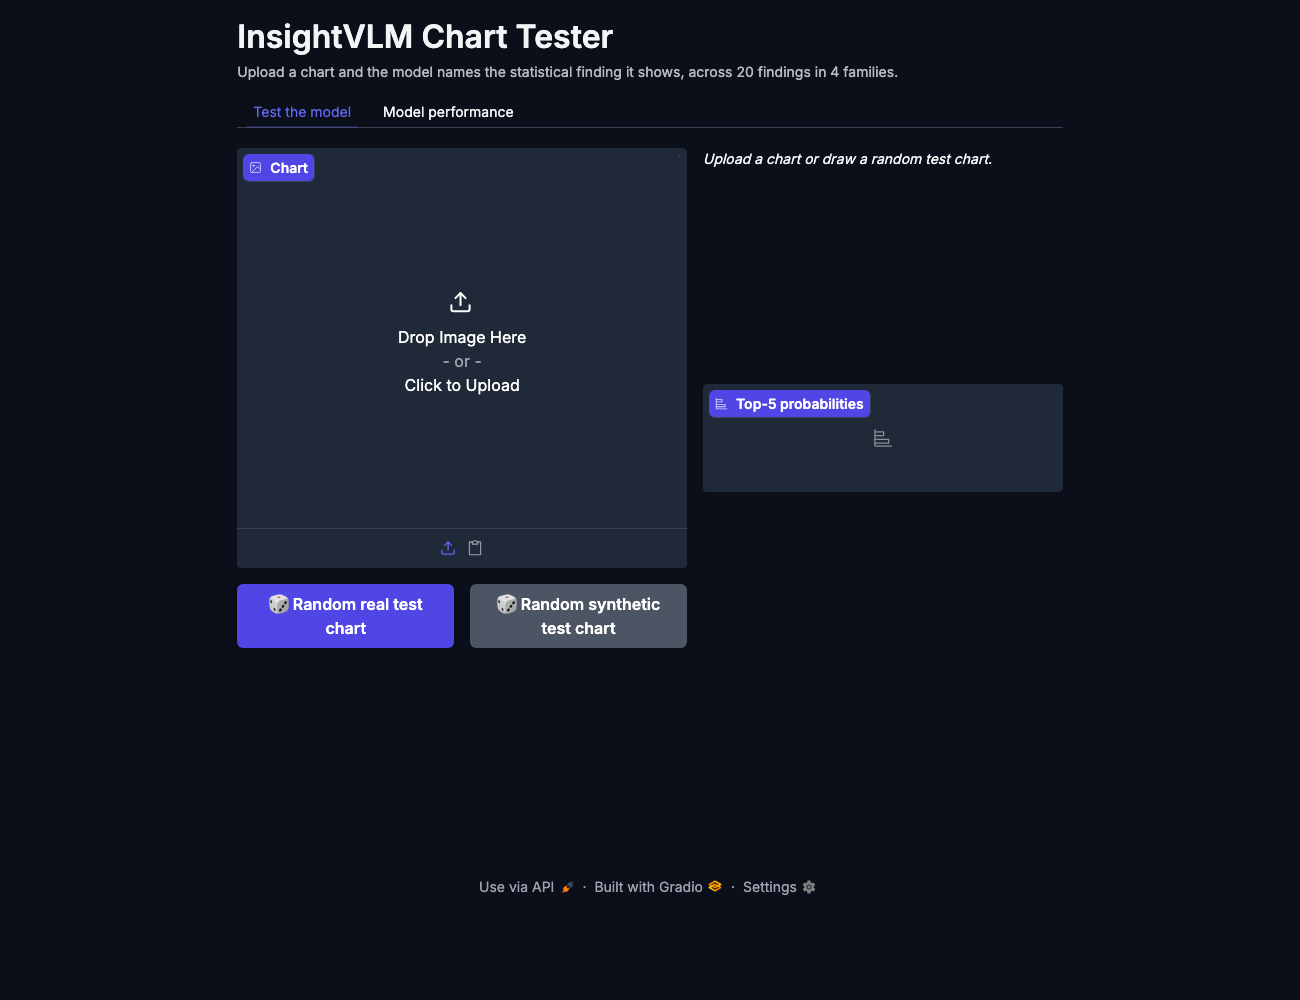
\includegraphics[width=0.85\linewidth]{app_home.png}
\caption{The tester's main tab. A chart can be uploaded, pasted from the clipboard, or
drawn at random from the held-out real or synthetic test charts.}
\label{fig:app}
\end{figure}

\paragraph{Running it.}
\begin{verbatim}
pip install torch torchvision gradio pandas pyarrow pillow
python app.py            # then open http://127.0.0.1:7860
\end{verbatim}

\paragraph{What it shows.} For an uploaded chart:
\begin{itemize}[leftmargin=1.3em]
  \item the predicted finding in plain language, its confidence, and its family;
  \item how many ensemble members agree;
  \item the definition of the finding and the statistical test that licenses it;
  \item the five most probable findings;
  \item a warning when confidence is below 50\%, since the chart may show a mix of
  patterns or one outside the 20 classes.
\end{itemize}
The \emph{random real test chart} and \emph{random synthetic test chart} buttons draw a
held-out test chart, predict it, and show the verified ground truth, its source, chart
type, difficulty and verified insight beside the prediction, marked correct or wrong.
The \emph{Model performance} tab lists the ensemble's test accuracy on real and synthetic
charts against the zero-shot baselines and the no-pixel floor.

\paragraph{Limits.} The tester classifies into the 20 known findings only. Charts from
tools unlike the training renderers are less reliable (Section~\ref{sec:rq4}), and
compound findings are reported as a single class.

\chapter{Artefacts and Reproduction}
\label{app:repro}

Every number in this thesis is produced by a script in the project repository
(Table~\ref{tab:repro}). Training ran on Kaggle (two T4 GPUs) from notebooks generated
by \texttt{train/make\_split\_notebooks.py}; everything else runs on a laptop CPU or
Apple-silicon GPU.

\begin{table}[h]\centering\small
\caption{Where each result comes from.}
\label{tab:repro}
\begin{tabular}{p{5.2cm}p{9.0cm}}
\toprule
\textbf{Result} & \textbf{Command or file} \\
\midrule
Dataset build and audit & \texttt{python run\_all.py}; \texttt{build/07\_validate.py}; \texttt{build/10\_bias\_audit.py} \\
Clean (version-2) renders & \texttt{build/06\_render.py --clean} \\
Supplementary real pool & \texttt{build/12\_extra\_real.py}, then \texttt{06\_render.py --records cache/records\_extra.jsonl} \\
Plotly / Vega-Lite test renders & \texttt{build/11\_render\_plotly.py}; \texttt{build/13\_render\_vega.py} \\
Augmentation renders & \texttt{11\_render\_plotly.py --split train}; \texttt{06\_render.py --randstyle} \\
Model training & notebooks \texttt{nb5\_real}, \texttt{nb5x\_*}, \texttt{nb7\_*} \\
Zero-shot VLM baselines & notebooks \texttt{nb6\_zeroshot}, \texttt{nb6b\_zeroshot\_ts} \\
Leak ablation (Table~\ref{tab:leak}) & \texttt{train/ablate\_marks.py} \\
Probabilities per model and renderer & \texttt{train/cache\_probs.py [--view plotly|vega]} \\
Deployed ensemble & \texttt{train/final\_ensemble.py} $\rightarrow$ \texttt{results/final\_ensemble.json} \\
Main table, CIs, McNemar & \texttt{train/stats\_report.py} $\rightarrow$ \texttt{results/stats\_report.json} \\
Grounding (Table~\ref{tab:grounding}) & \texttt{train/grounding\_eval.py} $\rightarrow$ \texttt{results/grounding.json} \\
Figures & \texttt{paper/make\_figures.py} \\
Human label check (Table~\ref{tab:labelcheck}) & \texttt{train/human\_study\_eval.py} (answers and key kept private) \\
\bottomrule
\end{tabular}
\end{table}

\paragraph{Data.} InsightVLM-20K version 2 is on Kaggle
(\texttt{asifxzaman/insightvlm-20k-v2}), with the supplementary pool
(\texttt{insightvlm-extra-real}) and the augmentation renders
(\texttt{insightvlm-aug-train}). The datasheet (\texttt{DATASHEET.md}) and audit report
(\texttt{BIAS\_AUDIT.md}) ship with the data.
              % A: interactive tester, B: artefacts and reproduction

\end{document}
